\begin{frame}
    \frametitle{Advice to a supplicant}
	
	\begin{itemize}
		\item Figure out the likelihood function
		\item Figure out how to maximize while being as lazy as possible
		\begin{itemize}
			\item No hand calculation of partial derivatives of complicated LL fcn
			\item Minimize or eliminate programming
			\item Communicate the method to our student correspondent
		\end{itemize}
		\item Take advantage of widely available software\pause {\color{red} ---Excel!}
		\bigskip
		\item Excel has a built-in black-box maximizer
		\item Excel produces reasonably close to ET Table~3 (but occasional differences in second significant digit)\pause
		\bigskip
		\item Who's right? (Excel not known for outstanding numerics)
		\item Also: \emph{\color{red} Excel spreadsheets are the opposite of reproducible}
	\end{itemize}
\end{frame}

\begin{frame}
	\frametitle{And the answer is\dots.}
	\begin{center}
		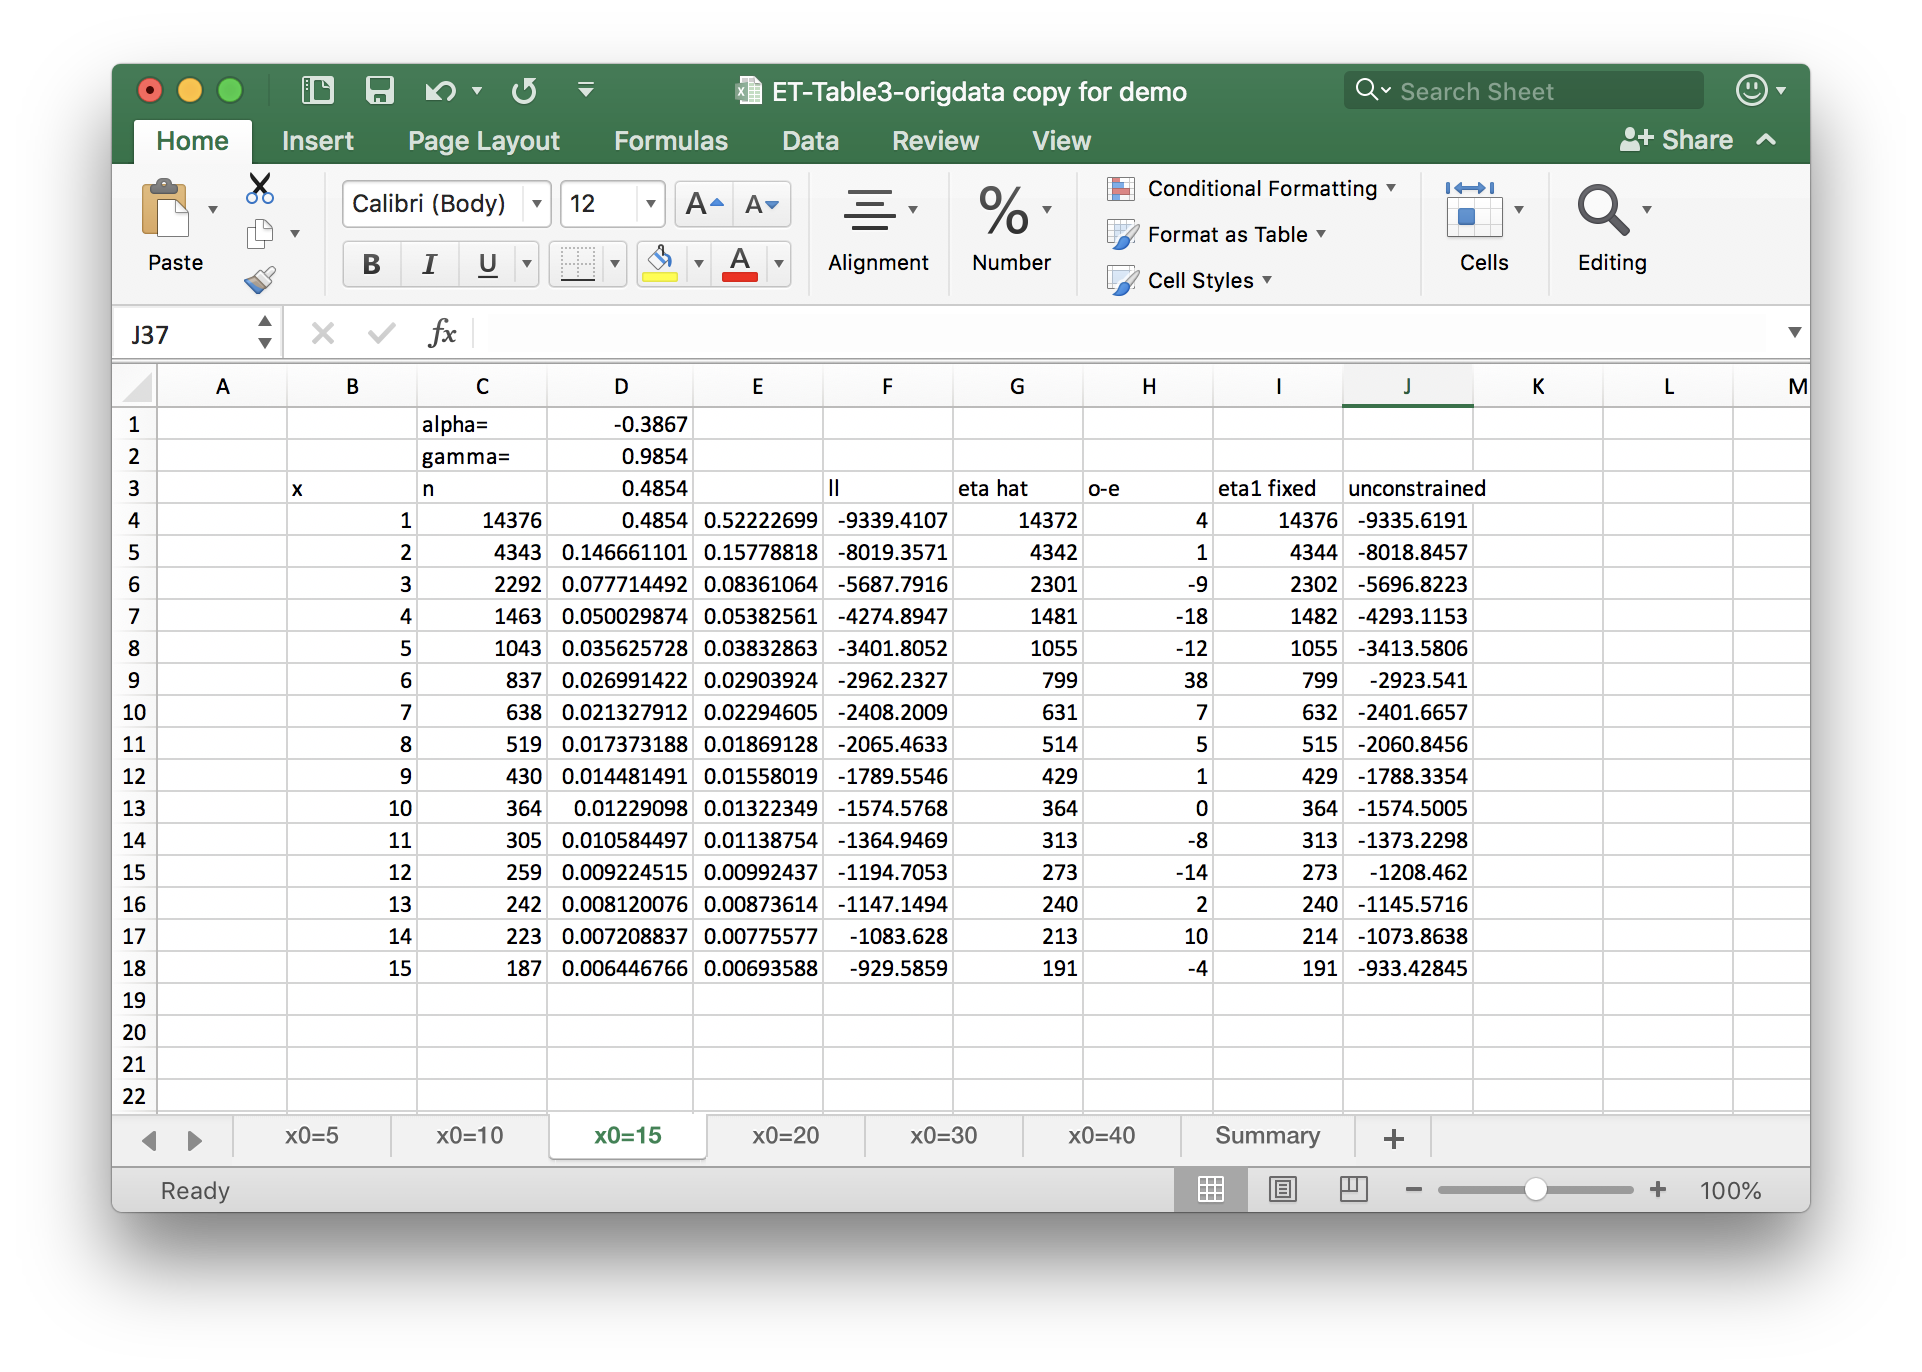
\includegraphics[width=4.5in]{../Manuscripts/Photos/Excel-x0=15.png}
	\end{center}
	
\end{frame}